The following analysis takes places outside of the processor I developed, using python scripts to analyse the data stored in the produced root file. This data was generated by choosing the best of all 3 ${E}_{\gamma}$ solutions, with  ${m}_{\gamma} = {m}_{\nu} = 0$. Unless otherwise explicitly stated, I did not cheat the beam background removal but I did include the boost into the centre of mass frame.
\\\\
Before any analysis I make sure that I am looking only at the muon signal, as this is the focus of my analysis, by making a cut on the events in MC collection that produced a muon.

%---------------------------------------------------------------------------------------------------------------------------------------------------------%---------------------------------------------------------------------------------------------------------------------------------------------------------
\subsection{Cut Flow}
\label{SUBSEC:CutFlow}

I sequentially apply all of the same cuts as in Ivan’s thesis \cite{IvanMarchesini} to obtain a cut flow histogram, which tests the efficiency of each of the cuts. This histogram is created by dividing the number of events left after each cut by the initial number of events considered as signal. I can then compare my results to Ivans to see how my processor and the particle reconstruction is performing compared to him. I did this for two different statistical sample sizes, the higher statistics sample being the sample I have used throughout the rest of this report. Further, I created the flow diagram again by cheating the beam background removal, and by applying the additional initial cut that the ISR energy is small (${E}_{\gamma}^{MC} < 1$ GeV). The final plot was made to see if the ISR made a considerable contribution to the efficiency of the cuts.
\\\\
There are a few subtle differences between the cuts that Ivan and I made, due to the reconstruction methods we implemented. The first was the cut on the jet reconstruction variables ${y}_{+}$ and ${y}_{-}$. I made FastJets reconstruct two jets, corresponding to the 2 quarks, and physically this is the minimum number of jets that occur, as we cannot create a single quark. This means the cut on the ${y}_{-}$ variable that Ivan makes is unphysical in my analysis. Ivan applies this cut because he also considered final states with 4 quarks. The lepton cut that I make is also different to Ivan’s. I am using an IsolatedLeptonTaggingProcessor, and so make the cut that a single isolated lepton is reconstructed. There are a considerable number of events where the processor reconstructs zero particles, and so this cut can be significant. Ivan on the other hand is using a jet reconstruction processor with a specific energy cut to reconstruct isolated leptons. The final difference is that Ivan makes a 'charged lepton' cut, which I cannot see a description of in his thesis. I do not make a similar cut and so the efficiencies of my results will not change in this cut.
\\\\
For convenience the cuts and efficiencies are tabulated in Table.~\ref{TAB:SelectionEfficiencies}, and the resulting total flow diagram can be seen in (Figure.~\ref{FIG:Flow}).
\\\\
\begin{table}[!]
    \centering
    \caption{
        Selection efficiency of sequantially applied cuts. Where the post ISR correction ${m}_{W}^{lep}$ was calculated using all 3 possible ${E}_{\gamma}$ solutions. (*) Indicates cuts where my and Ivan's cuts differ, as discussed in the text.
    }
    \resizebox{0.8\textwidth}{!}{%
    \begin{tabular}{|l|l|l|l|l|l|} \hline
        Order & Cut description & \multicolumn{4}{c|}{Efficiency [\%]} \\ \cline{3-6}
        & & \multicolumn{3}{c|}{My Results} & Ivan's Results \\  \cline{3-5}
        & & n = 2129 & \multicolumn{2}{c|}{n = 99419} & n = 107233 \\ \cline{4-5}
        & & & no cheat & cheat & \\ \hline \hline
        0 & muon signal & 100.00 & 100.00 & 100.00 & 100.00 \\ \hline
        1 & track multiplicity\tablefootnote{track mulitplicity was taken as the number of reconstructed charged particles.} ${n}_{tracks} \ge 10$ & 97.13 & 97.01 & 96.23 & 99.996 \\ \hline
        2 & center of mass energy $\sqrt{s} > 100$ GeV & 92.29 & 91.69 & 84.35 & 97.96 \\ \hline
        3 & total transverse momentum ${P}_{T} > 5$ GeV & 91.16 & 90.47 & 83.28 & 96.69 \\ \hline
        4 & total energy ${E}_{SUM} < 500$ GeV & 89.66 & 89.28 & 82.70 & 95.36 \\ \hline
        5 & $\ln{({y}_{+})} \in [-12, -3]$ (*) & 88.69 & 88.08 & 82.47 & 95.01 \\ \hline
        6 & 1 lepton found (*) & 80.65 & 80.77 & 81.50 & 78.75 \\ \hline
        7 & pre ISR correction ${m}_{W}^{lep} \in [20, 250]$ GeV &  78.23 & 77.94 & 77.84 & 76.61 \\ \hline
        8 & tau discrimination\tablefootnote{${\tau}_{discr}$ defined by ${\tau}_{discr} = {(\frac{2{E}_{lep}}{\sqrt{s}})}^{2} + {(\frac{{m}_{W}^{lep}}{{m}_{W}^{true}})}^{2}$} &  76.05 & 75.60 & 75.73 & 74.07 \\ \hline
        9 & charged lepton (*) & 76.05 & 75.60 & 75.73 & 73.51 \\ \hline
        10 & isolation variable\tablefootnote{$\Delta{\Omega}_{iso}$ defined as,
        \begin{align}
            ({\phi}_{lep} - {\phi}_{had}) < \pi \to \Delta{\Omega}_{iso} &= \sqrt{{({\theta}_{lep} - {\theta}_{had})}^{2}+{({\phi}_{lep} - {\phi}_{had})}^{2}} \\
            ({\phi}_{lep} - {\phi}_{had}) \ge \pi \to \Delta{\Omega}_{iso} &= \sqrt{{({\theta}_{lep} - {\theta}_{had})}^{2} + {(2\pi - |{\phi}_{lep} - {\phi}_{had} |)}^{2}} \, .
        \end{align}} ${\Delta\Omega}_{iso} > 0.5$ & 76.01 & 75.58 & 75.72 & 73.42 \\ \hline
        11 & post ISR correction ${m}_{W}^{lep} \in [40, 120]$ GeV & 72.90 & 72.77 & 72.33 & 70.13 \\ \hline
        12 & post ISR correction ${m}_{W}^{had} \in [40, 120]$ GeV & 63.21 & 62.92 & 70.52 & 66.93 \\ \hline
        13 & $\cos{{\theta}_{W}} > -0.95$ & 63.02 & 62.65 & 70.21 & 66.78 \\ \hline
        \end{tabular}
        }
        \label{TAB:SelectionEfficiencies}
    \end{table}

\begin{figure}[!]
    \centering
    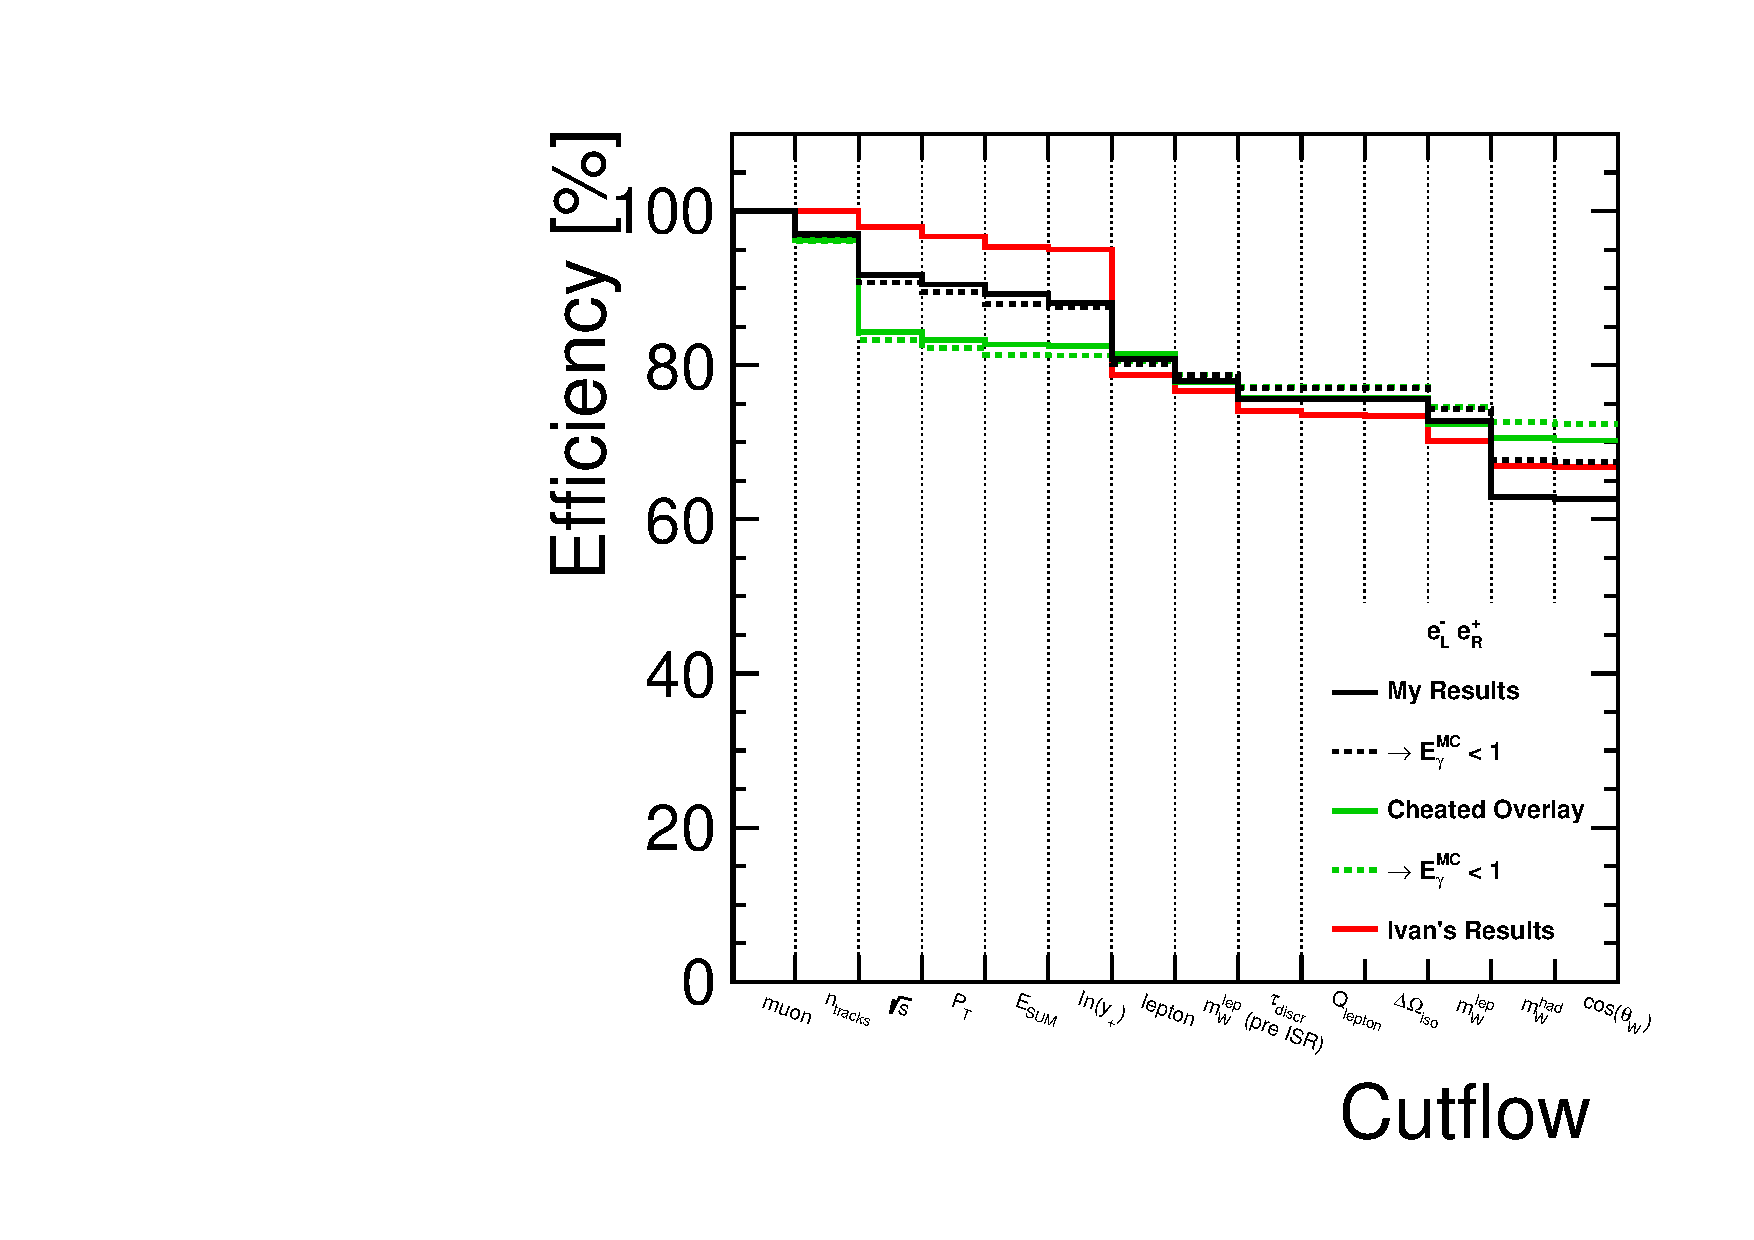
\includegraphics[width=0.8\textwidth]{\imagepath/P_HistFlow3_All.pdf}
    \caption{
    Histograms showing the cut flows for Ivan's results, my results (with and whithout cheating overlay removal), and my results again when the ISR photon has low energy (${E}_{\gamma} < 1$). The cuts on the x axis are as defined in Table.~\ref{TAB:SelectionEfficiencies}.
    }
    \label{FIG:Flow}
\end{figure}

We can see a fairly large difference in the cut efficiencies before the lepton cut. I believe this is because, for me, the cut on finding only one isolated lepton would make a considerable difference to the performace of the reconstruction. In all of the events where no isolated leptons were reconstructed the leptonic W boson is reconstructed entiely from the invisble neutrino, which will be completely wrong. We see that 'My Results' and the 'Cheated Overlay' reconverge on this lepton cut and I believe this is because the differences prior were caused by such events. I have not explored this further in this report, a check would be to perform the lepton cut first and see how the two historgams differ then.
\\\\
After the lepton cut, we can see that my results are generally performing better than Ivan's, untill the cut on the ${m}_{W}^{had}$ where it is considerably worse. By looking at the cheated results though we can see that this is apparently due to the beam background. We also see that after the lepton cut the ${E}_{\gamma}^{MC} < 1$ GeV is consistently performing better than the full signal, which suggests that large ISR energies worsens the performance of the reconstruciton.

%---------------------------------------------------------------------------------------------------------------------------------------------------------%---------------------------------------------------------------------------------------------------------------------------------------------------------
\subsection{Angle Cut Efficiencies}
\label{SUBSEC:AngleCutEfficiencies}
I can now complete the end goal of my report, to evaluate the angular dependancy of the cut efficiency. This can be done by dividing an angular distribution histogram with all of the perviously defined cuts applied, by the same histogram where the only applied cut is that we are looking at a muon signal. I did this for both the full signal and the ${E}_{\gamma}^{MC} < 1$ GeV signal, which can be seen in Figure.~\ref{FIG:AngleEfficiencies}.
\\
\begin{figure}
    \begin{subfigure}[t]{0.32\textwidth}
        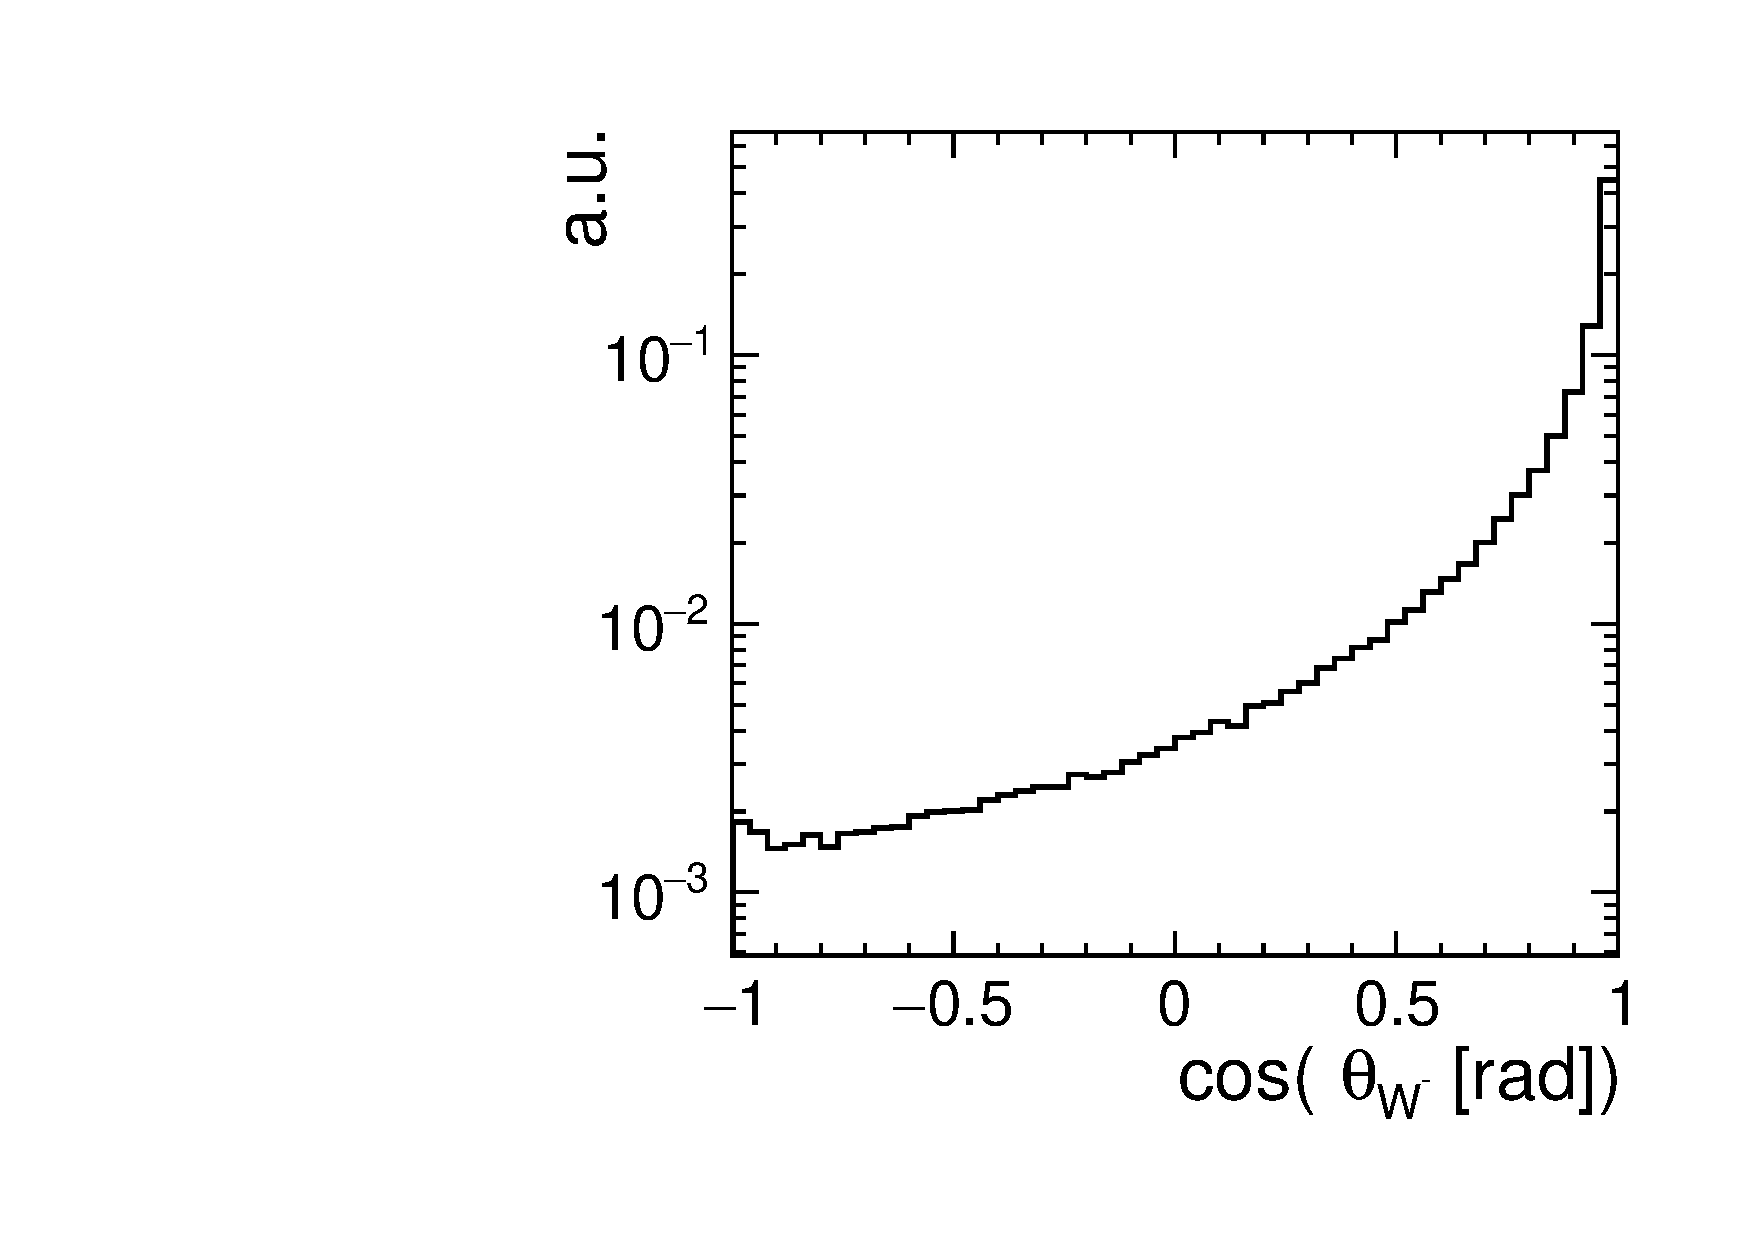
\includegraphics[width=\textwidth]{\imagepath/ThetaMin_cos.pdf}
        \caption{}
        \label{SUBFIG:ThetaMin}
    \end{subfigure}
    \begin{subfigure}[t]{0.32\textwidth}
        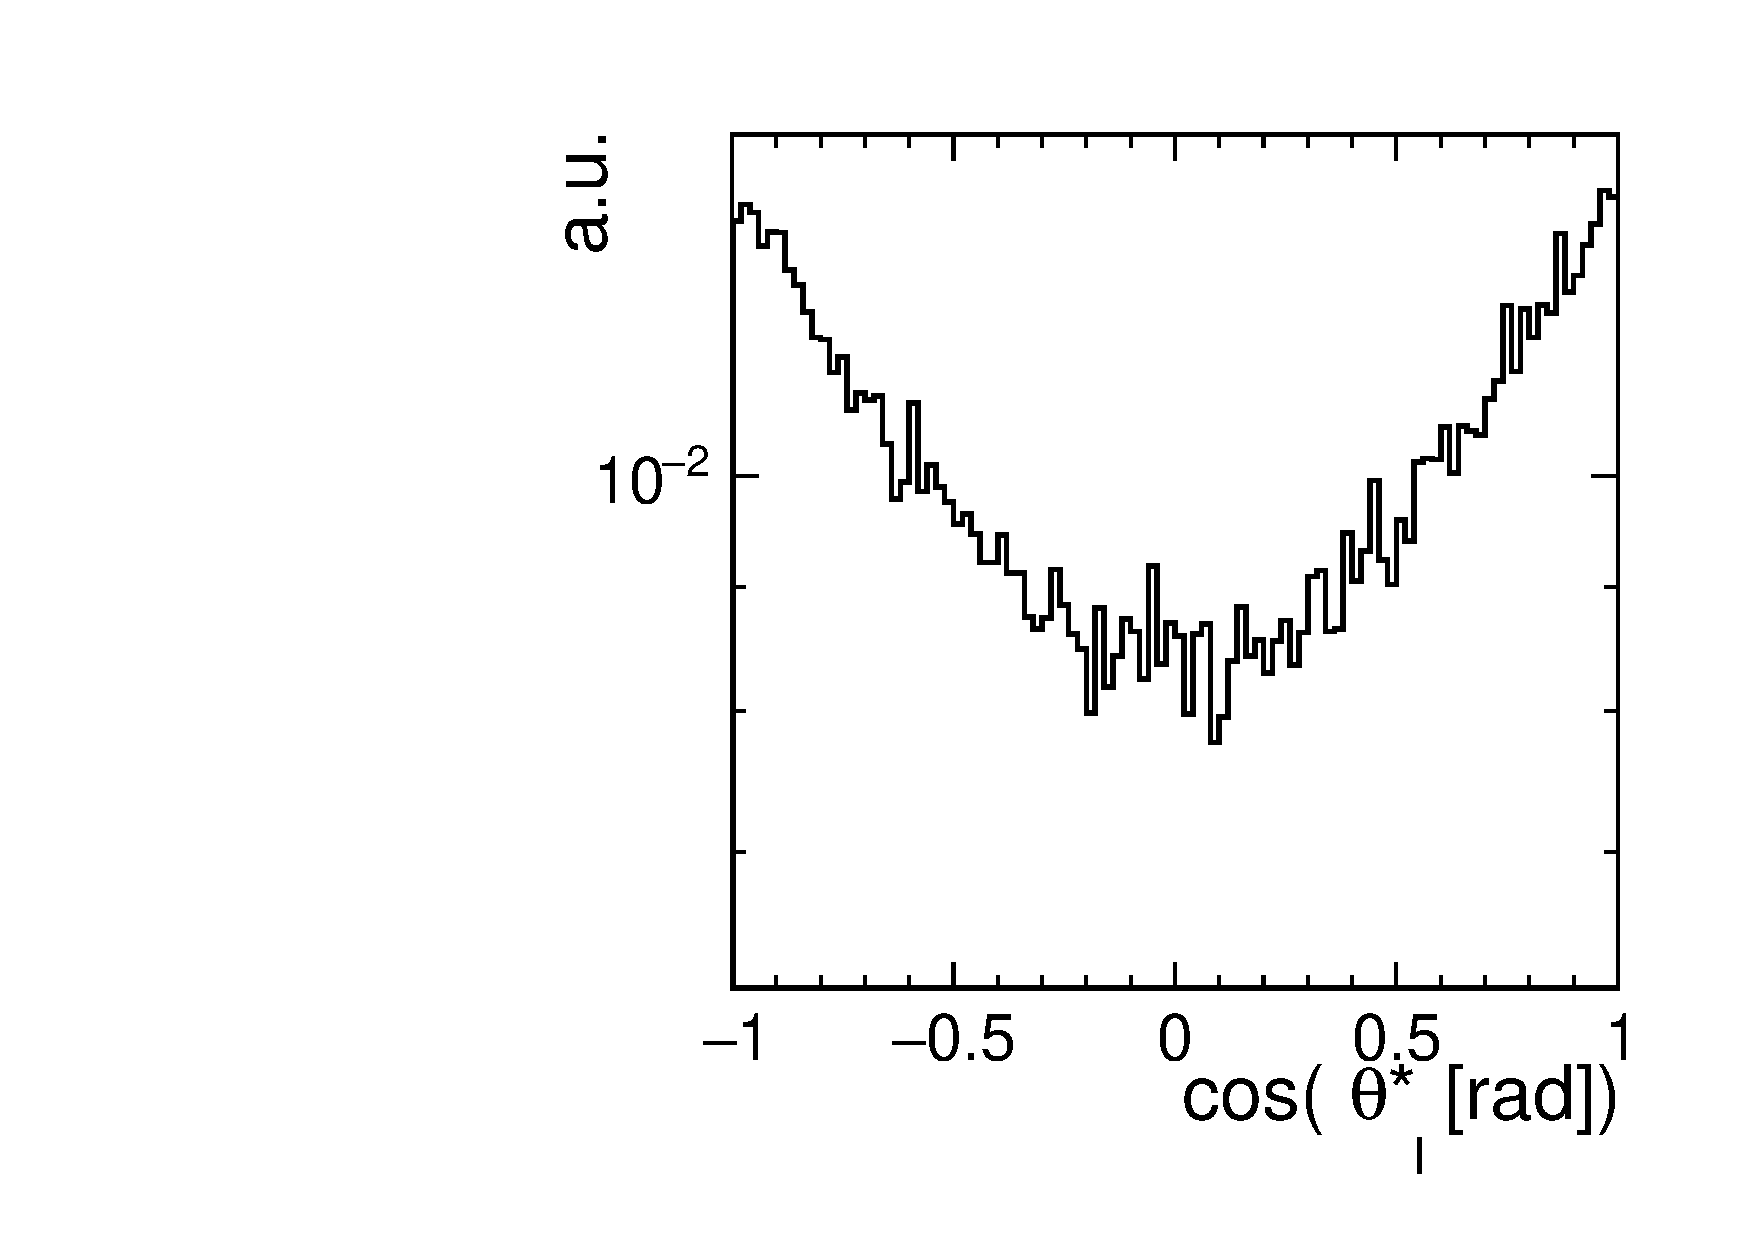
\includegraphics[width=\textwidth]{\imagepath/ThetaLep_cos.pdf}
        \caption{}
        \label{SUBFIG:ThetaLep}
    \end{subfigure}
    \begin{subfigure}[t]{0.32\textwidth}
        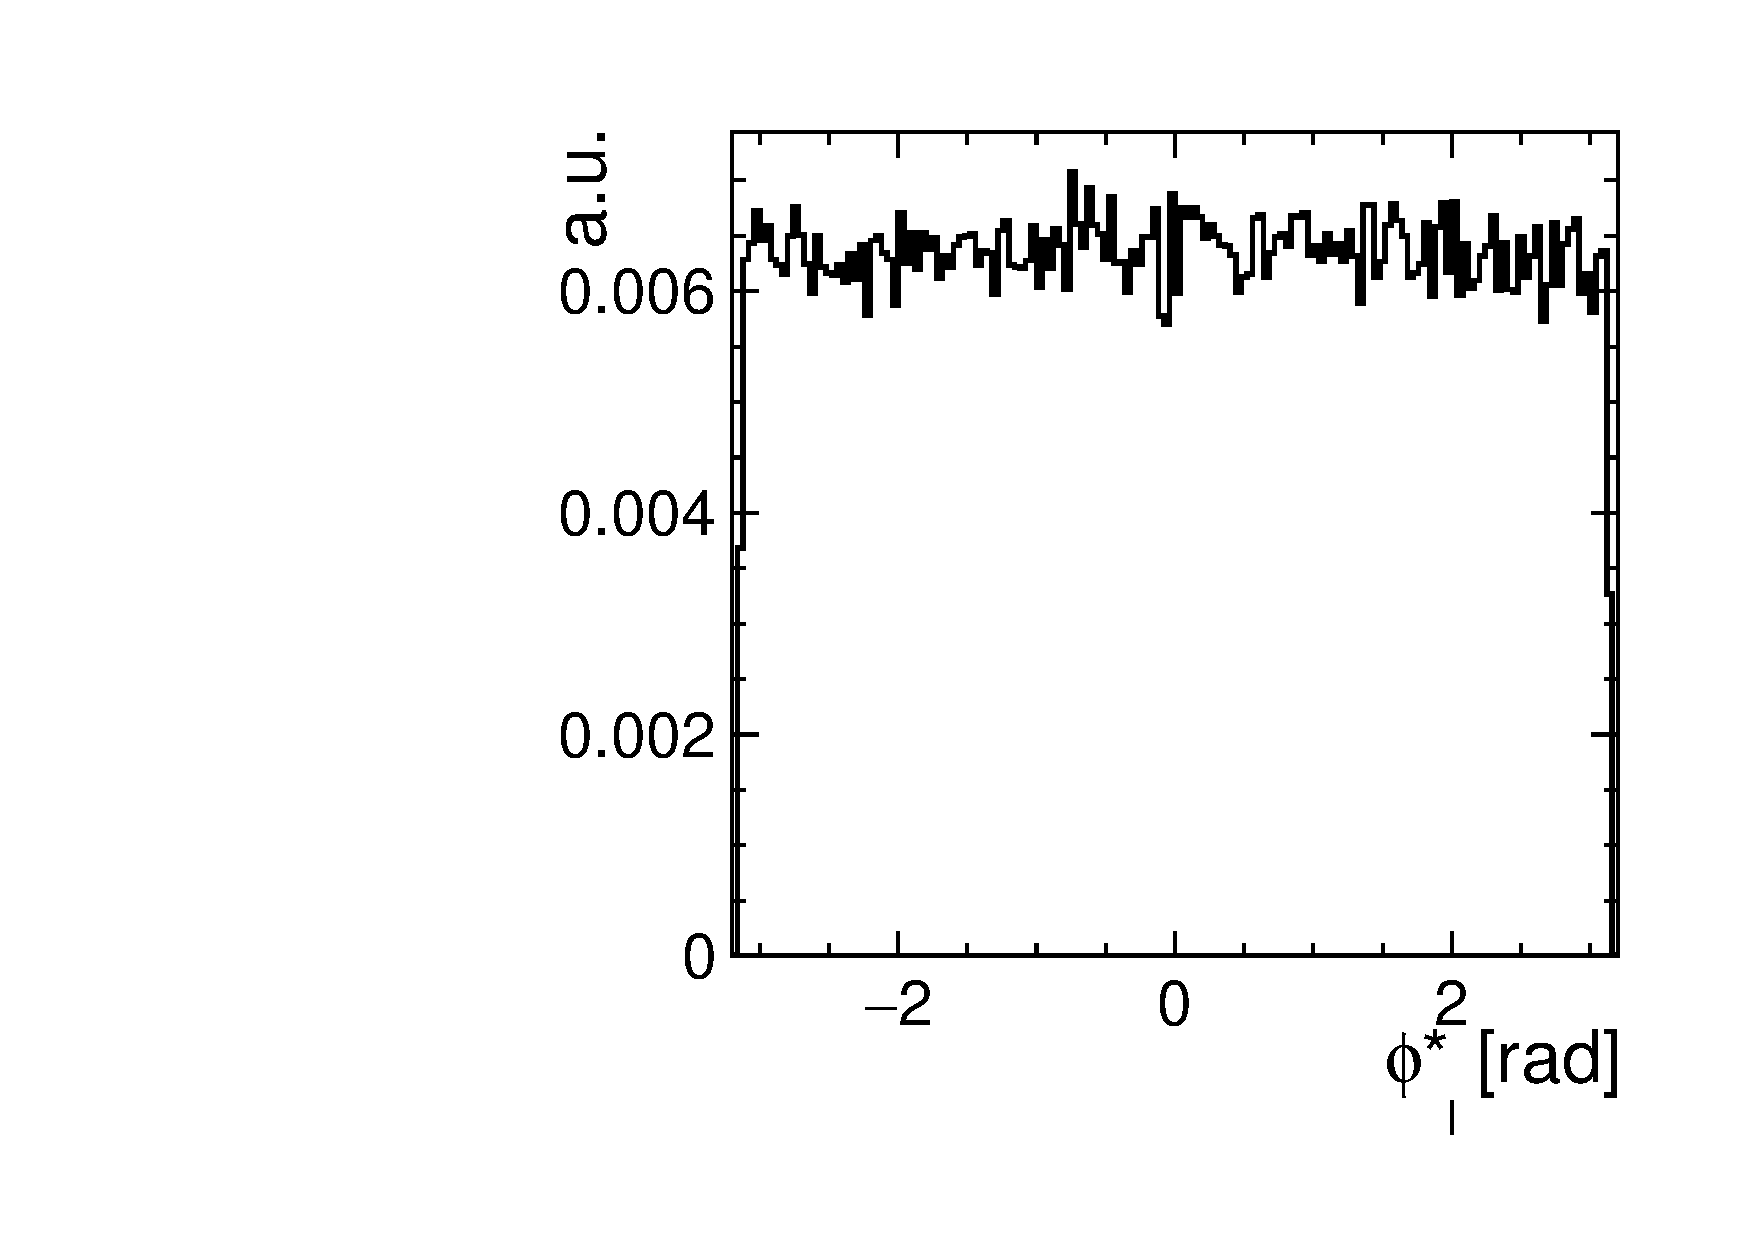
\includegraphics[width=\textwidth]{\imagepath/PhiLep.pdf}
        \caption{}
        \label{SUBFIG:PhiLep}
    \end{subfigure}\\
    \begin{subfigure}[t]{0.32\textwidth}
        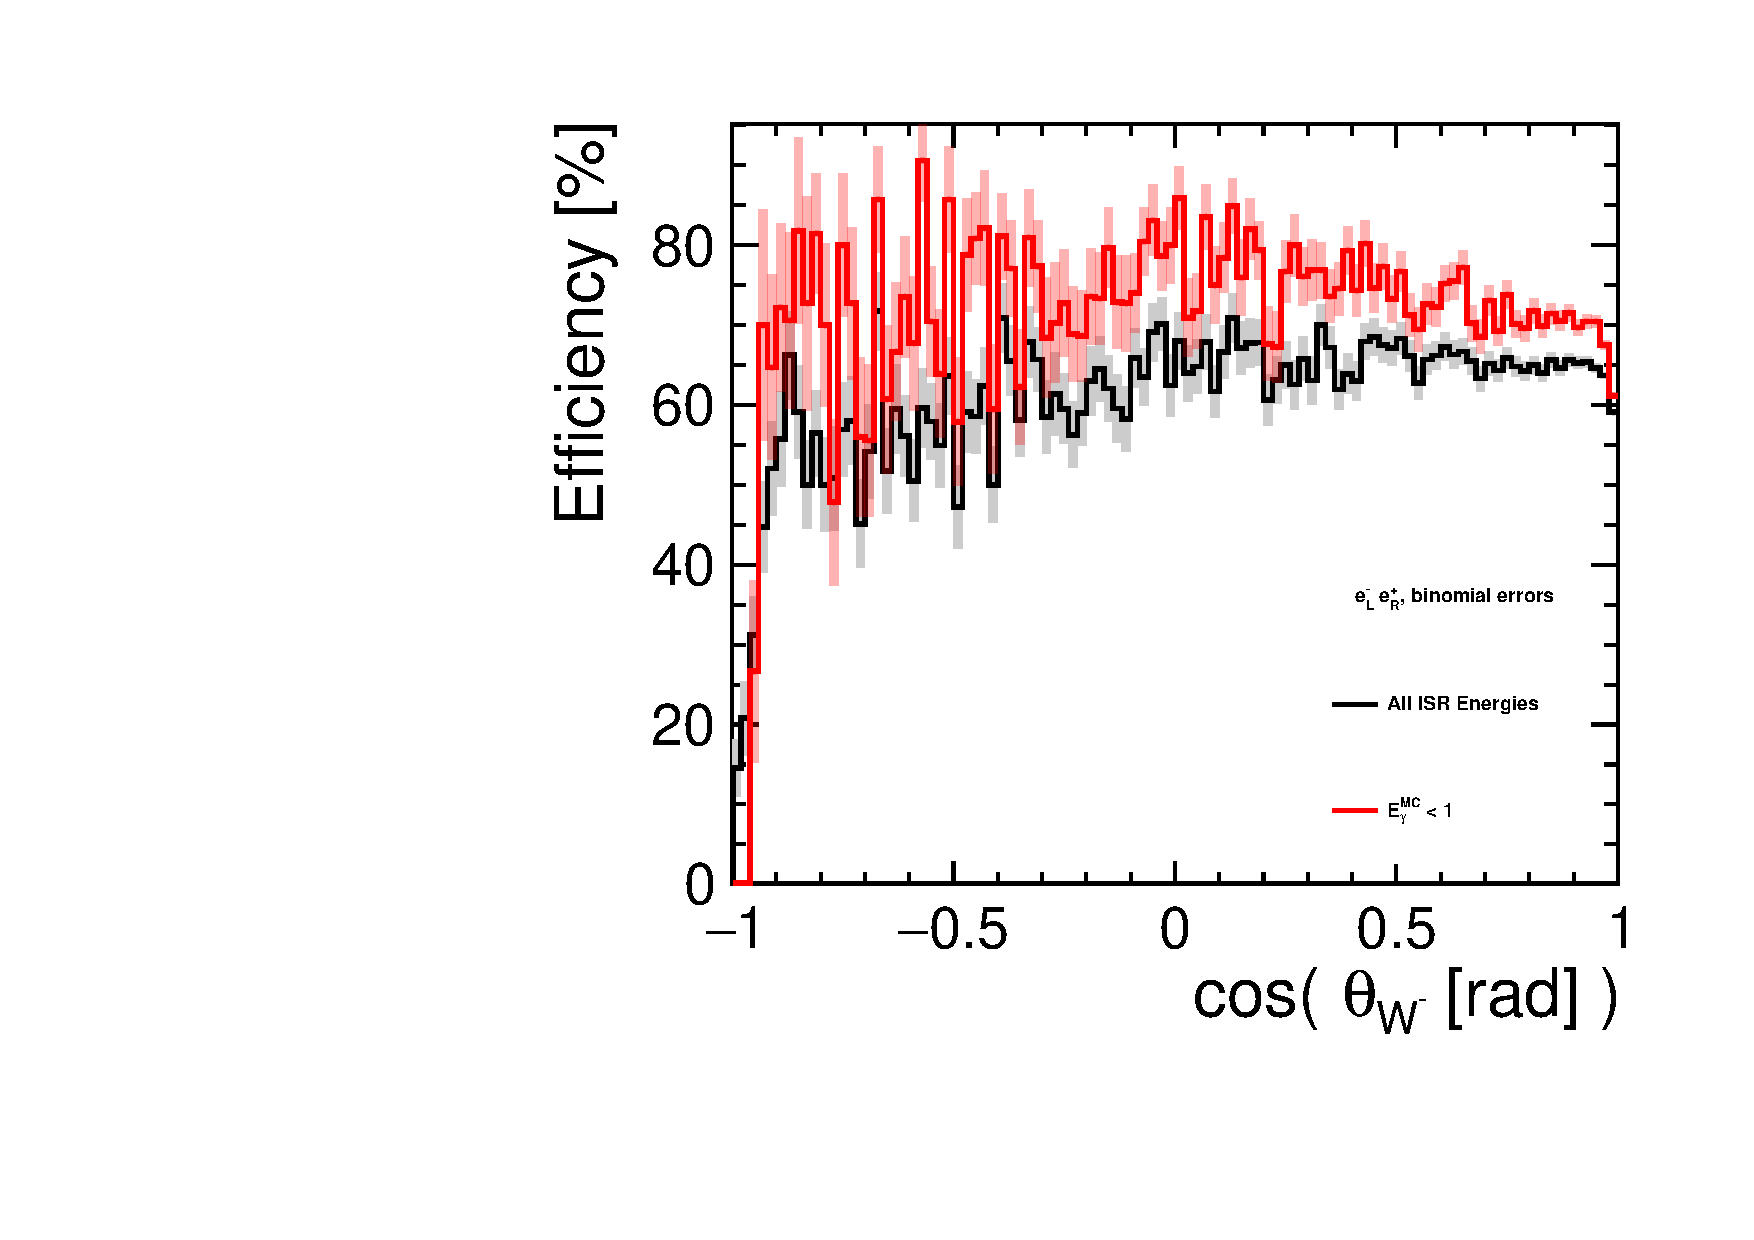
\includegraphics[width=\textwidth]{\imagepath/P_E_ThetaMin_cos_err_Both.pdf}
        \caption{}
        \label{SUBFIG:ThetaMinError}
    \end{subfigure}
    \begin{subfigure}[t]{0.32\textwidth}
        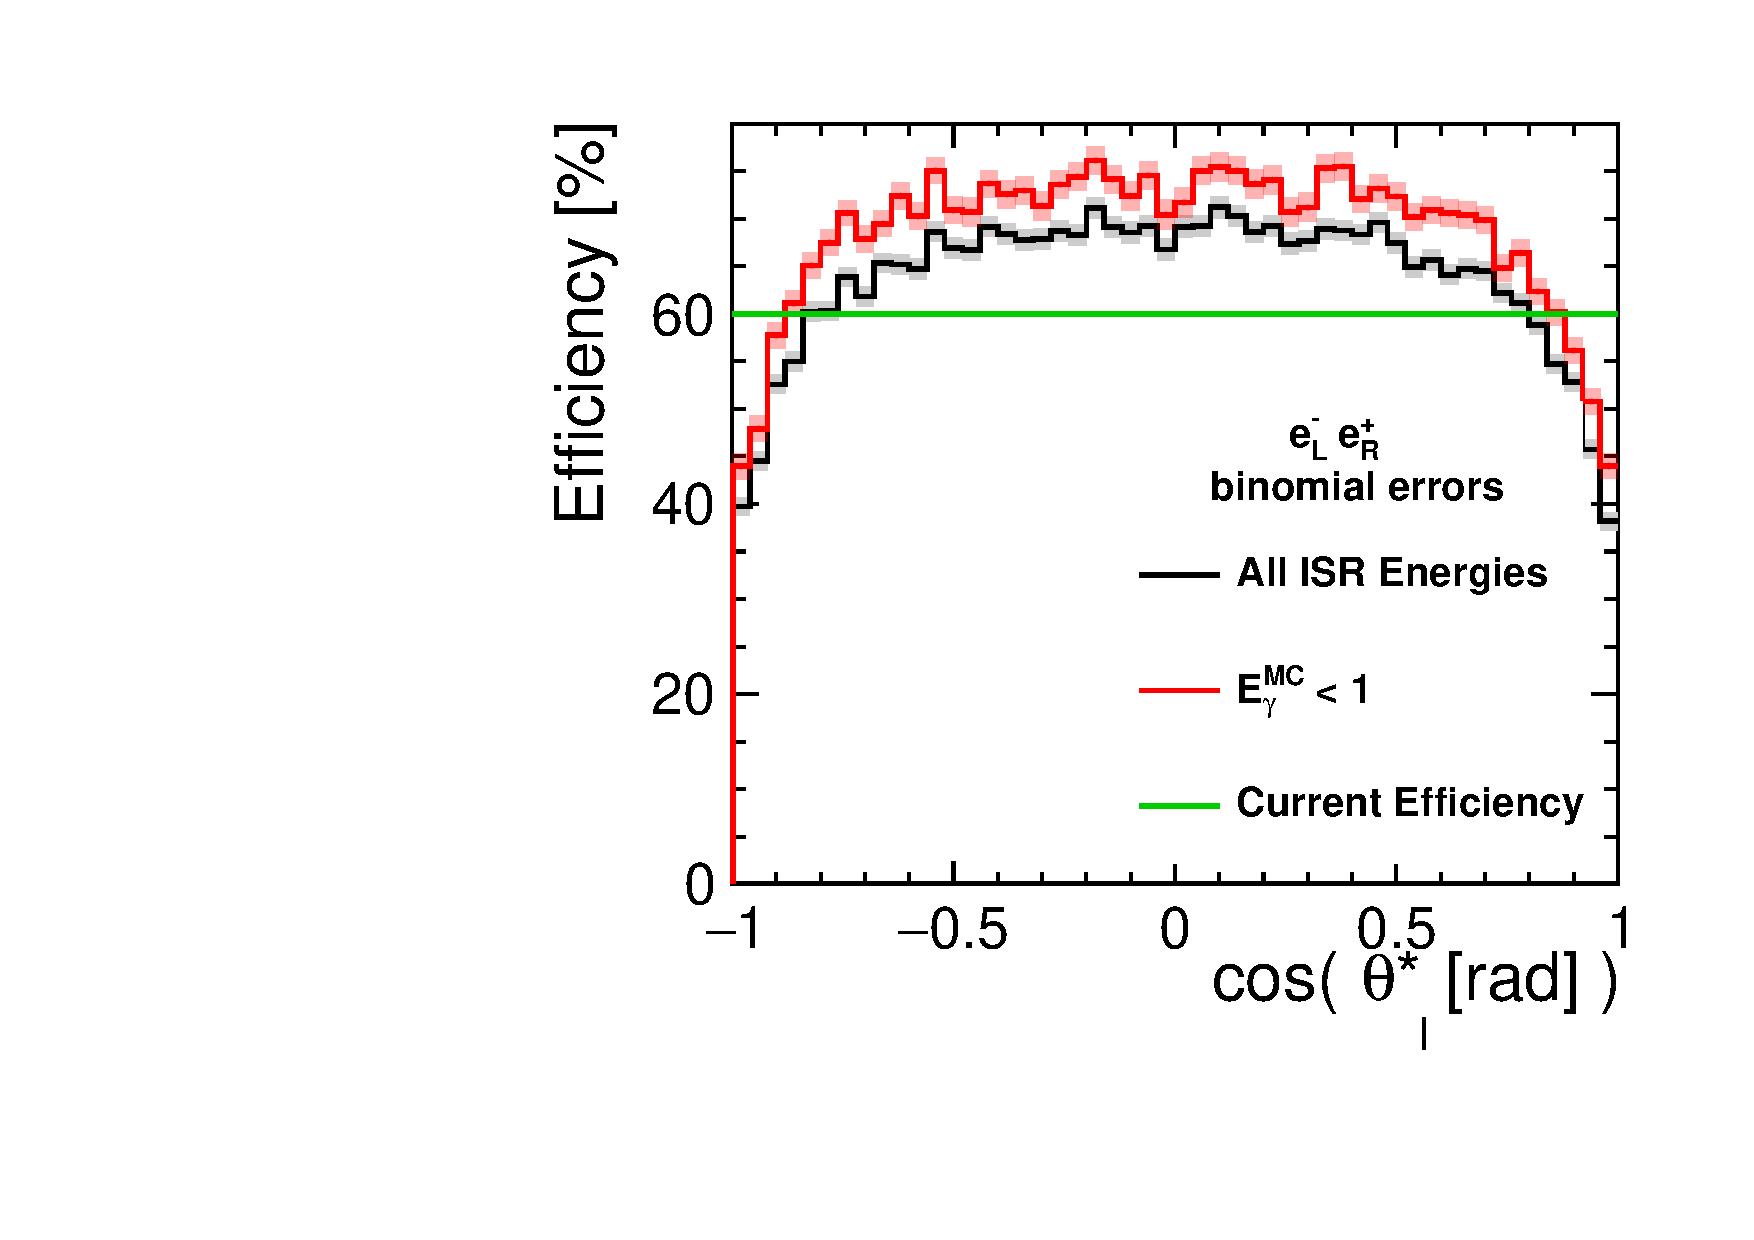
\includegraphics[width=\textwidth]{\imagepath/P_E_ThetaLep_cos_err_Both.pdf}
        \caption{}
        \label{SUBFIG:ThetaLepError}
    \end{subfigure}
    \begin{subfigure}[t]{0.32\textwidth}
        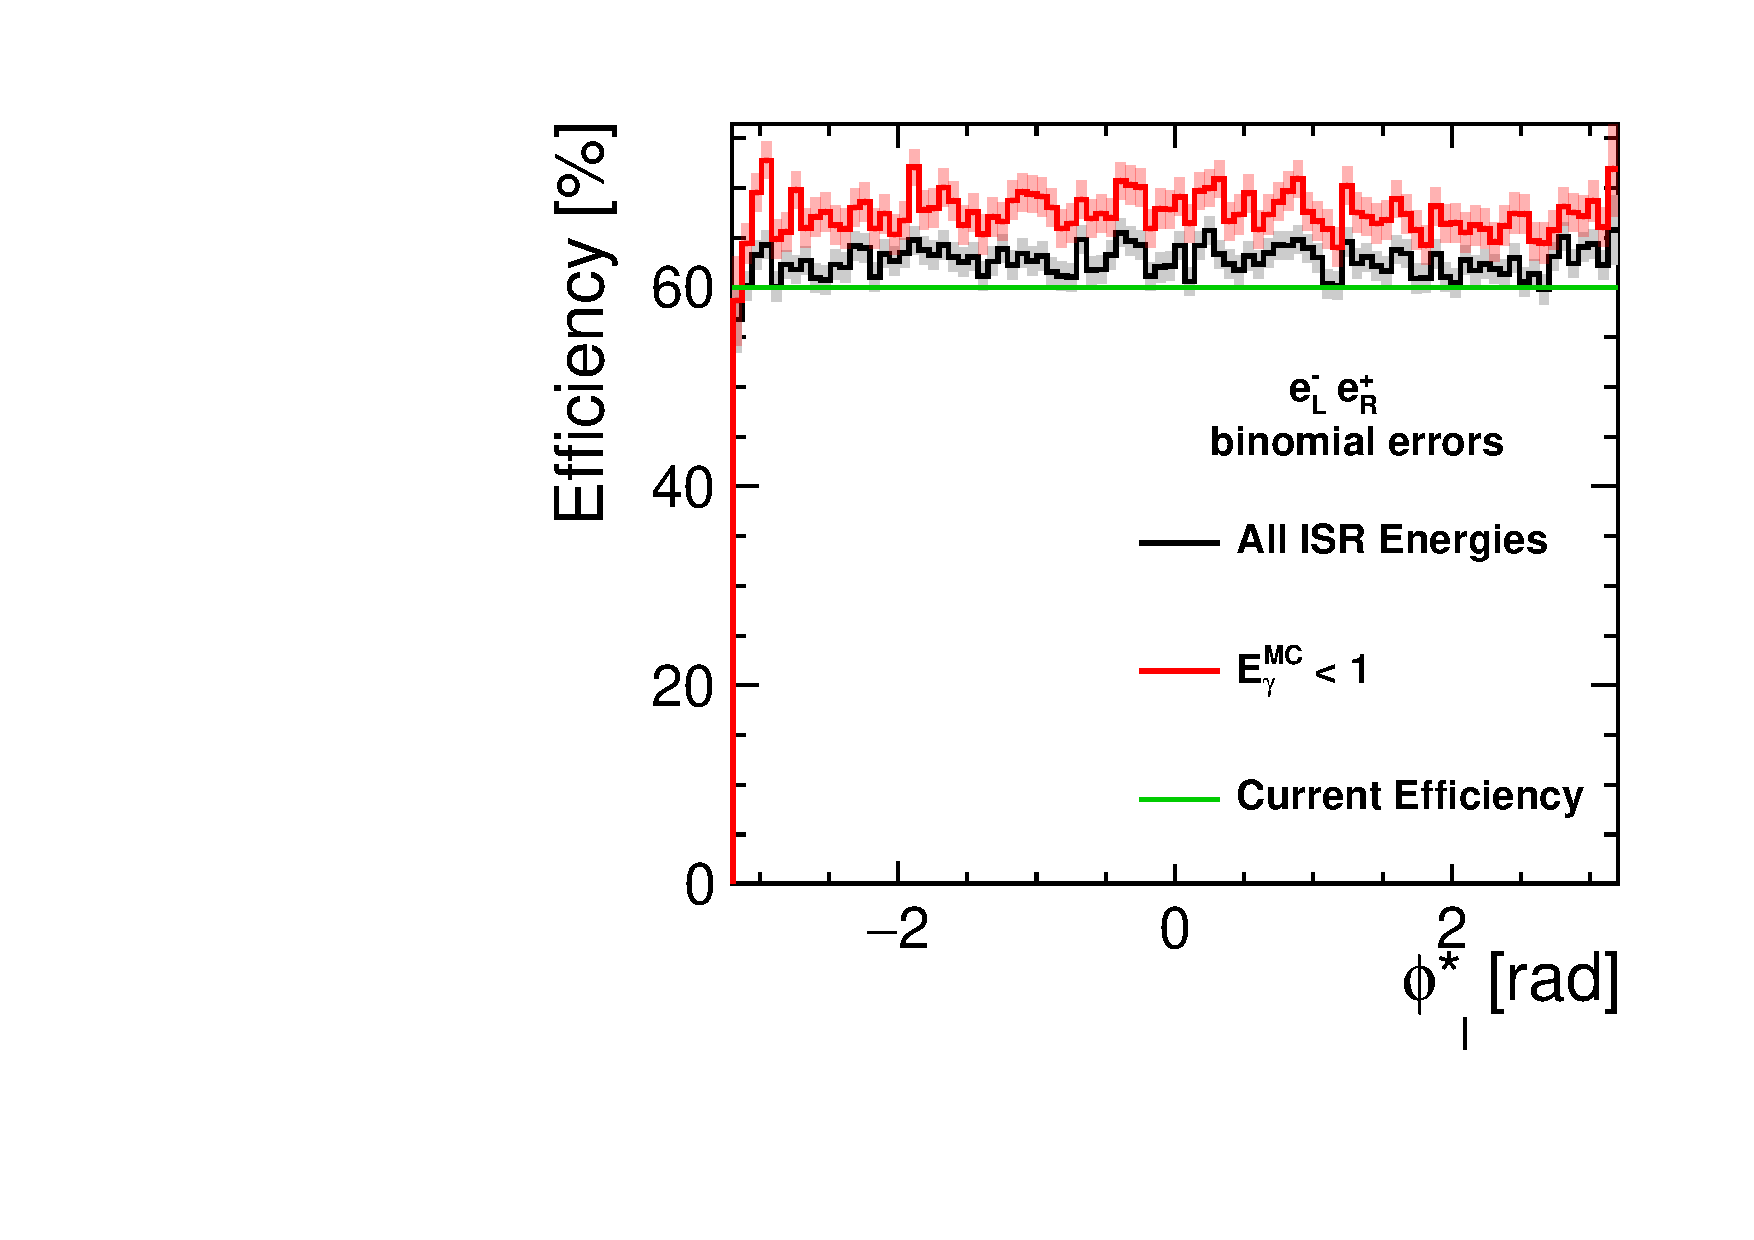
\includegraphics[width=\textwidth]{\imagepath/P_E_PhiLep_err_Both.pdf}
        \caption{}
        \label{SUBFIG:PhiLepError}
    \end{subfigure}
    \caption{
    \subfigref{SUBFIG:ThetaMin}, \subfigref{SUBFIG:ThetaLep} and \subfigref{SUBFIG:PhiLep} are the extracted angles as defined in Figure.~\ref{FIG:Angles}. \\
    \subfigref{SUBFIG:ThetaMinError}, \subfigref{SUBFIG:ThetaLepError} and \subfigref{SUBFIG:PhiLepError} are the associated cut efficiencies, after applying the cuts outlined in Table.~\ref{TAB:SelectionEfficiencies}.
    }
    \label{FIG:AngleEfficiencies}
\end{figure}

The $\cos{({\theta}_{{W}^{-}})}$ plot can be seen to be fairly statistically limited towards -1, in the backwards direction, and this greatly reduces the efficiency here, it is however reasonably constant throughout the rest of the distribution. The $\cos{({\theta}_{l}^{*})}$ appears to have a poor efficiency in regions closely aligned to the beam-pipe. This is as expected due to ***FILL ME****. ${\phi}_{l}^{*}$ has a uniform efficiency as well as angular distribution. This is to be expected because there is no initial phi momentum that could bias this result. Even though the lepton's angle will have a dependance on that of the W boson it decayed from, this W boson will be uniformly distributed in phi and so we expect the same from the lepton. This  may not be the case if the stared (*) coordinate system what oriented such that ${\phi}_{l}^{*} = 0$ lied in the plane defined by the beam axis and the W boson, but that has not been explored in this report.
\\\\
The ${E}_{\gamma}^{MC} < 1$ GeV signal performed very similarly to the full signal, but the magnitude of the efficiency seemed to be different by a reasonably consistent factor.
